%% 
%% Copyright 2007-2020 Elsevier Ltd
%% 
%% This file is part of the 'Elsarticle Bundle'.
%% ---------------------------------------------
%% 
%% It may be distributed under the conditions of the LaTeX Project Public
%% License, either version 1.2 of this license or (at your option) any
%% later version.  The latest version of this license is in
%%    http://www.latex-project.org/lppl.txt
%% and version 1.2 or later is part of all distributions of LaTeX
%% version 1999/12/01 or later.
%% 
%% The list of all files belonging to the 'Elsarticle Bundle' is
%% given in the file `manifest.txt'.
%% 
%% Template article for Elsevier's document class `elsarticle'
%% with harvard style bibliographic references

%\documentclass[preprint,12pt,authoryear]{elsarticle}

%% Use the option review to obtain double line spacing
%% \documentclass[authoryear,preprint,review,12pt]{elsarticle}

%% Use the options 1p,twocolumn; 3p; 3p,twocolumn; 5p; or 5p,twocolumn
%% for a journal layout:
%% \documentclass[final,1p,times,authoryear]{elsarticle}
%% \documentclass[final,1p,times,twocolumn,authoryear]{elsarticle}
%% \documentclass[final,3p,times,authoryear]{elsarticle}
%% \documentclass[final,3p,times,twocolumn,authoryear]{elsarticle}
%% \documentclass[final,5p,times,authoryear]{elsarticle}
 \documentclass[final,5p,times,twocolumn,authoryear]{elsarticle}

%% For including figures, graphicx.sty has been loaded in
%% elsarticle.cls. If you prefer to use the old commands
%% please give \usepackage{epsfig}

%% The amssymb package provides various useful mathematical symbols
\usepackage{amssymb}
\usepackage{lipsum}
%% The amsthm package provides extended theorem environments
%% \usepackage{amsthm}

%% The lineno packages adds line numbers. Start line numbering with
%% \begin{linenumbers}, end it with \end{linenumbers}. Or switch it on
%% for the whole article with \linenumbers.
%% \usepackage{lineno}

%% You might want to define your own abbreviated commands for common used terms, e.g.:
\newcommand{\kms}{km\,s$^{-1}$}
\newcommand{\msun}{$M_\odot}

\journal{Dr. Amin Faraji}


\begin{document}

\begin{frontmatter}

%% Title, authors and addresses

%% use the tnoteref command within \title for footnotes;
%% use the tnotetext command for theassociated footnote;
%% use the fnref command within \author or \affiliation for footnotes;
%% use the fntext command for theassociated footnote;
%% use the corref command within \author for corresponding author footnotes;
%% use the cortext command for theassociated footnote;
%% use the ead command for the email address,
%% and the form \ead[url] for the home page:
%% \title{Title\tnoteref{label1}}
%% \tnotetext[label1]{}
%% \author{Name\corref{cor1}\fnref{label2}}
%% \ead{email address}
%% \ead[url]{home page}
%% \fntext[label2]{}
%% \cortext[cor1]{}
%% \affiliation{organization={},
%%            addressline={}, 
%%            city={},
%%            postcode={}, 
%%            state={},
%%            country={}}
%% \fntext[label3]{}

\title{Exploring Periodic Boundary Conditions: A Study on 2D and 3D Spheres and Continuum Limit}

%% use optional labels to link authors explicitly to addresses:
%% \author[label1,label2]{}
%% \affiliation[label1]{organization={},
%%             addressline={},
%%             city={},
%%             postcode={},
%%             state={},
%%             country={}}
%%
%% \affiliation[label2]{organization={},
%%             addressline={},
%%             city={},
%%             postcode={},
%%             state={},
%%             country={}}

\author[first]{Alireza Same}
\fntext[first]{99100709}
\ead{alirezasame@gmail.com}
\author[second]{Hanie Hatami}
\fntext[second]{99100614}
\ead{alirezasame@gmail.com}
\author[third]{Mehrnaz Rabiee}
\fntext[third]{99100669}
\ead{alirezasame@gmail.com}

\begin{abstract}
%% Text of abstract
Example abstract for the Annals of Physics journal. Here you provide a brief summary of the research and the results.
\end{abstract}

%%Graphical abstract
%\begin{graphicalabstract}
%\includegraphics{grabs}
%\end{graphicalabstract}

%%Research highlights
%\begin{highlights}
%\item Research highlight 1
%\item Research highlight 2
%\end{highlights}

\begin{keyword}
%% keywords here, in the form: keyword \sep keyword, up to a maximum of 6 keywords
keyword 1 \sep keyword 2 \sep keyword 3 \sep keyword 4

%% PACS codes here, in the form: \PACS code \sep code

%% MSC codes here, in the form: \MSC code \sep code
%% or \MSC[2008] code \sep code (2000 is the default)

\end{keyword}


\end{frontmatter}

%\tableofcontents

%% \linenumbers

%% main text

\section{Introduction}
\label{introduction}

\section{1D Spheres Revisited}
\label{sec-1D}
As it is done in many standard textbooks (see \cite{georgiPhysicsWaves2015}), the simple case of modeling a disturbance through a circular rod can be first modeled by considering two fundamental assumptions: Firstly, Interactions is only between neighboring particles. They cannot have a significant effect on far away neighbors, this property is what makes studying waves interesting. Secondly, the force between particles is approximately linear with respect to change of distance relative to their equilibrium distance. Although these two conditions make such great restrictions on the model that we are studying. It is rather accurate in the relatively accurate measurements made.

Consider a circle of radius $R$ with $N$ particles with same mass $m$ evenly distributed on the circle. With the assumptions made we can consider $N$ springs with spring constants $k$ identical to each other. This system experiences a symmetry called \textit{“Periodic Symmetry”}. As from rotation of $2\pi/N$ on either directions or reflections on either vertices we get the same system again. Our description should not make any distinction between these $2N$ cases. There is another free parameter in the  Question which is the initial position of on of the particles. As this is not measurable due to need for setting a starting point on circle we have all the information to describe the system. Figure \ref{fig-n4} shows the system for the special case $N=4$.

\begin{figure}
	\centering 
	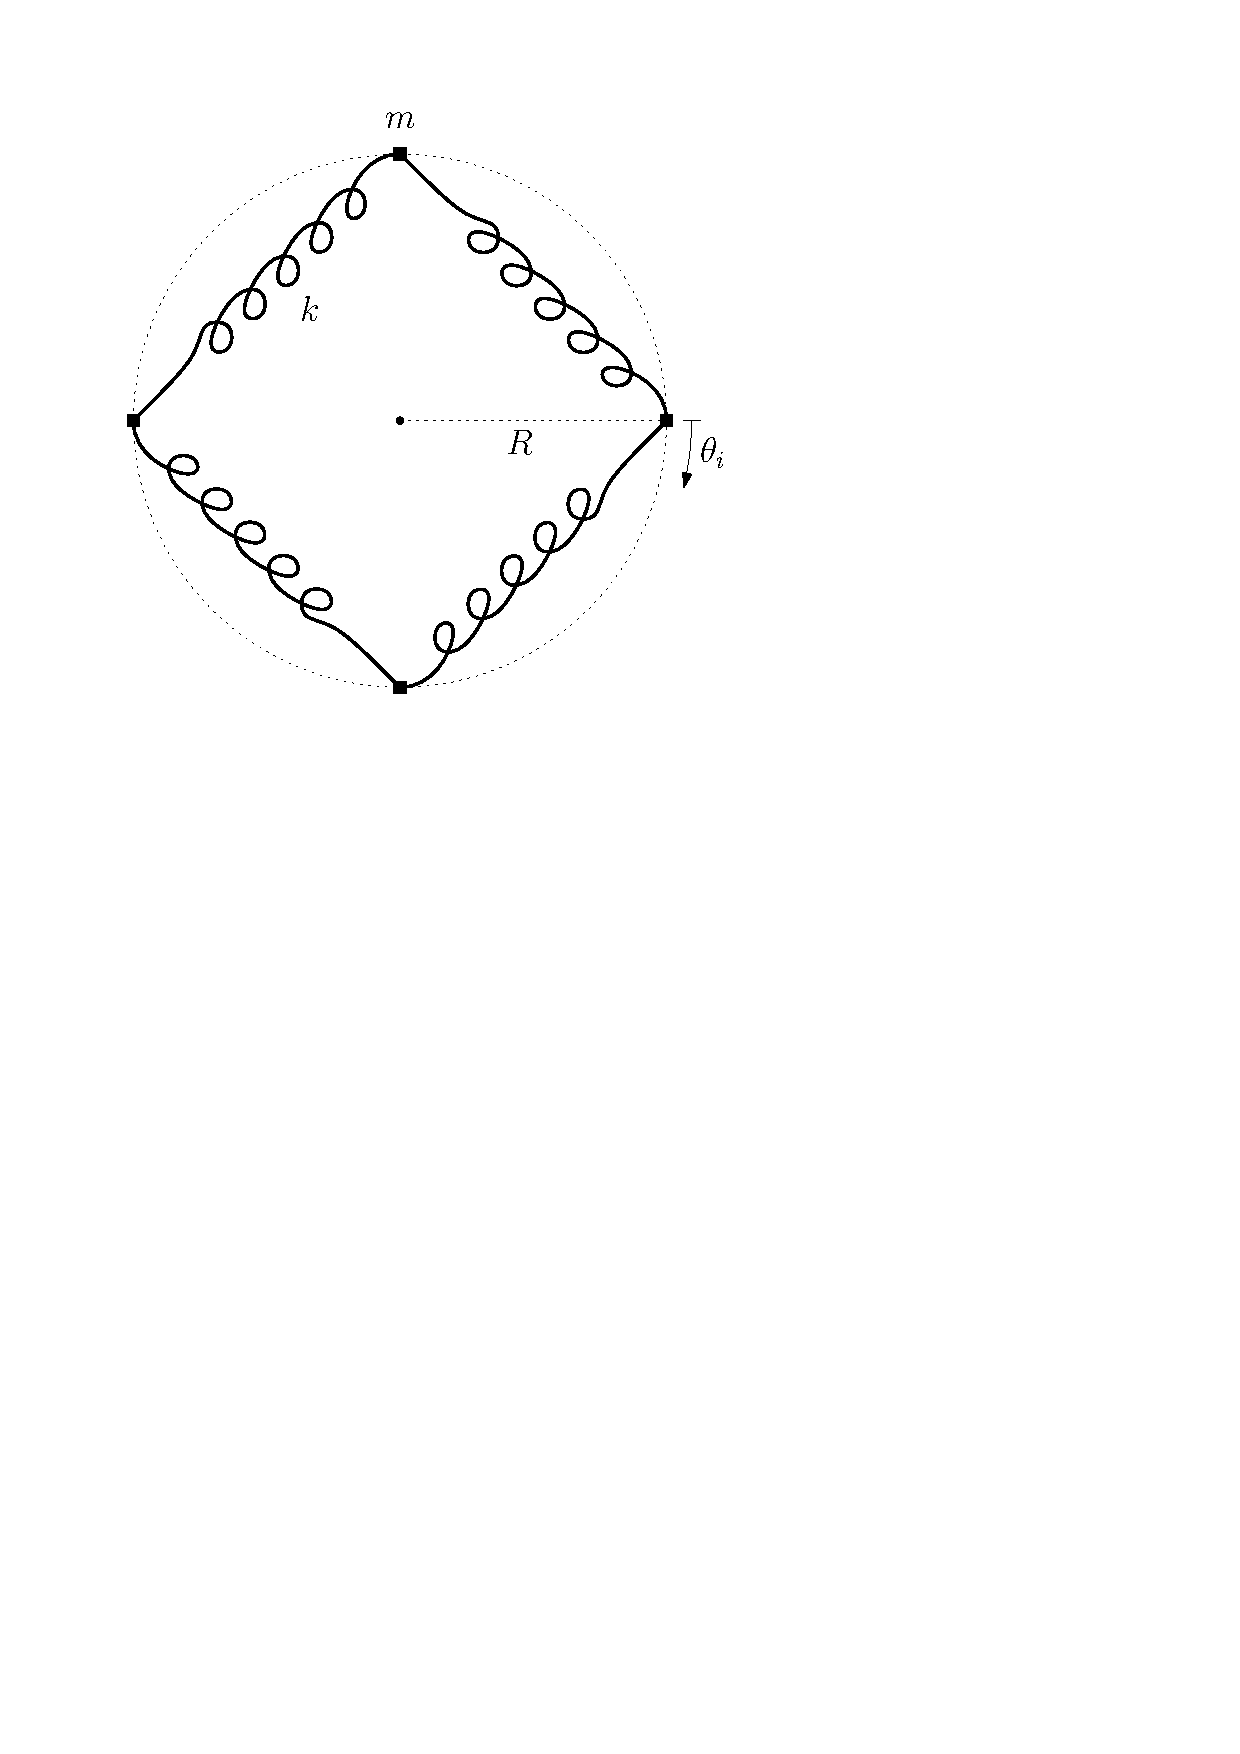
\includegraphics[width=0.25\textwidth]{../Figures/1D-4Particle-Springs.pdf}	
	\caption{4 identically distributed point masses on a circle} 
	\label{fig-n4}
\end{figure}

We want to derive the general formula for the N particle case from this simplified case.



\section{Discussion}
%%\label{}

\section{Summary and conclusions}
%%\label{}


\section*{Acknowledgements}
Thanks to ...

%% The Appendices part is started with the command \appendix;
%% appendix sections are then done as normal sections

%% If you have bibdatabase file and want bibtex to generate the
%% bibitems, please use
%%
\bibliographystyle{elsarticle-harv} 
\bibliography{zotero}

%% else use the following coding to input the bibitems directly in the
%% TeX file.

%%\begin{thebibliography}{00}

%% \bibitem[Author(year)]{label}
%% For example:

%% \bibitem[Aladro et al.(2015)]{Aladro15} Aladro, R., Martín, S., Riquelme, D., et al. 2015, \aas, 579, A101


%%\end{thebibliography}

\end{document}

\endinput
%%
%% End of file `elsarticle-template-harv.tex'.
